\documentclass[runningheads]{llncs}
\usepackage{mathptmx}            % Times, matching the report and the IEEE version
\usepackage[T1]{fontenc}
\usepackage[utf8]{inputenc}
\usepackage{graphicx,amsmath,amssymb,array,booktabs}
\usepackage[hidelinks]{hyperref}
\usepackage{color}
\begin{document}
\title{Prediction of Heart Disease using Ensemble Learning: A Reproducible Re-implementation and Multi-Dataset Evaluation of the MPBE Model}
\titlerunning{Heart Disease Prediction using Ensemble Learning}
\author{Salil Mahale}
\authorrunning{S. Mahale}
\institute{Department of Computer Engineering, St. Francis Institute of Technology, University of Mumbai, Mumbai, India\\
\email{salil.mahale@student.sfit.ac.in}}
\maketitle
\begin{abstract}
Early prediction of heart disease from routine clinical attributes is a well studied classification problem, yet published accuracies on the UCI Cleveland dataset range from below 75\% to above 97\%, largely because of differing evaluation protocols. This paper re-implements the MinMax normalized Pearson coefficient Bagging Ensemble (MPBE) proposed by Muthulakshmi et al., which combines bagged Decision Tree, Random Forest, Naive Bayes and Support Vector Machine members, and evaluates it under a leakage free protocol: stratified 10-fold cross validation with scaling fitted inside each fold, on both the Cleveland dataset (303 patients) and a combined five source UCI dataset (918 unique patients). MPBE is compared against six single classifiers and six other ensembles (homogeneous bagging, soft and hard voting, stacking, AdaBoost, gradient boosting and XGBoost). On Cleveland, MPBE reaches 82.46\% accuracy and ROC-AUC 0.912, statistically level with the best models, but the 95.33\% reported originally is not reproduced. On the combined dataset MPBE is the best model (80.84\% accuracy, ROC-AUC 0.884) and loses the least accuracy when the population becomes heterogeneous. An ablation shows the Pearson feature selection step changes accuracy by under 0.5 points. The results support heterogeneous bagging as a robust default for tabular clinical screening and argue for cross validated reporting over single split headline figures.
\keywords{Heart disease prediction \and Ensemble learning \and Bagging \and Stacking \and Boosting \and Pearson correlation \and Cross validation \and UCI Cleveland}
\end{abstract}
\section{Introduction}
Cardiovascular disease is the leading cause of death worldwide, and in India a quarter of heart related deaths occur before the age of forty \cite{r1}. Thirteen routinely collected attributes (age, sex, chest pain type, resting blood pressure, cholesterol, fasting blood sugar, resting ECG, maximum heart rate, exercise induced angina, ST depression, ST slope, fluoroscopy vessel count and thalassemia status) are cheap to obtain, and a classifier that predicts angiographic disease from them can act as a screening aid. The UCI Cleveland dataset \cite{r22} has been the standard benchmark for this task for three decades, and ensemble methods, which combine several learners to reduce variance or bias, are consistently reported to outperform single classifiers on it \cite{r8,r9,r14}.

Muthulakshmi et al. \cite{r1} proposed the \textbf{MPBE} model: MinMax normalisation, Pearson correlation feature selection, and a bagging ensemble whose members are a Decision Tree, a Random Forest, a Naive Bayes classifier and an SVM, aggregated by mean score. They reported 95.33\% accuracy. The paper leaves several details open (the correlation threshold, whether scaling was fitted before or after splitting, whether aggregation is soft or hard) and evaluates on a single dataset. Recent work has warned that many accuracies above 95\% on Cleveland arise from optimistic protocols or duplicate rows \cite{r11,r21}. This paper therefore asks: (i) what accuracy does MPBE reach under a strict cross validated protocol, (ii) how does it compare with voting, stacking and boosting ensembles, and (iii) does its advantage transfer to a larger, heterogeneous population?

Our contributions are a fully specified, scikit-learn compatible re-implementation of MPBE; a fourteen model comparison on two datasets with accuracy, precision, recall, F1 and ROC-AUC; an ablation of the feature selection step; and an honest reconciliation of our numbers with the original claim. Code, data preparation and figures are released with the paper.

\section{Related Work}
Table 1 summarises the twenty studies reviewed. Three themes emerge. First, \textbf{ensembles beat weak learners by a wide margin but strong learners by a narrow one}: Latha and Jeeva \cite{r9} measured gains of up to 7.3 points from majority voting over weak classifiers, whereas Karadeniz et al. \cite{r14} and Chandrasekhar and Peddakrishna \cite{r18} found boosting, stacking and soft voting only marginally ahead of tuned logistic regression. Second, \textbf{feature selection helps modestly}: Haq et al. \cite{r5}, Alim et al. \cite{r7} and Li et al. \cite{r15} all found that dropping cholesterol and fasting blood sugar costs nothing and occasionally helps. Third, \textbf{protocol dominates}: Ali et al. \cite{r11} reported 100\% for Random Forest on a Kaggle copy later shown to contain duplicates, Ahmad et al. \cite{r19} showed that grid search on a single split pushes several models towards 99\%, and Adekoya et al. \cite{r21} and Mienye and Jere \cite{r16} argue for nested cross validation, calibration and explanation as the criteria that matter for clinical use. Multi dataset evaluation, as in Doppala et al. \cite{r6} and Asif et al. \cite{r17}, is the approach adopted here.

\begin{table}[htbp]
\centering
\caption{Summary of the reviewed studies}
\scriptsize
\begin{tabular}{>{\raggedright\arraybackslash}p{0.052\textwidth}>{\raggedright\arraybackslash}p{0.052\textwidth}>{\raggedright\arraybackslash}p{0.196\textwidth}>{\raggedright\arraybackslash}p{0.372\textwidth}>{\raggedright\arraybackslash}p{0.258\textwidth}}
\hline
\textbf{Ref} & \textbf{Year} & \textbf{Dataset} & \textbf{Technique} & \textbf{Reported result} \\
\hline
{}\cite{r2} & 2022 & Cleveland (UCI) & Multilayer Perceptron and K-Nearest Neighbour & MLP 82.47\% accuracy, AUC 86.41\% \\
{}\cite{r3} & 2022 & Cleveland (UCI) & Random Forest, KNN, Decision Tree, XGBoost plus a stacked ensemble and K-modes clustering & Stacked model reported 88.7\% accuracy \\
{}\cite{r4} & 2020 & Cleveland and Framingham & Homogeneous ensemble of CART trees combined by an accuracy based weighted aging classifier & 93\% on Cleveland, 91\% on Framingham \\
{}\cite{r5} & 2018 & Cleveland (UCI) & Seven classifiers (LR, KNN, ANN, SVM, NB, DT, RF) with Relief, mRMR and LASSO feature selection under 10-fold CV & Logistic Regression with Relief features 89\% accuracy \\
{}\cite{r6} & 2022 & Cleveland, Statlog and a Mendeley cardiovascular dataset & Majority voting and stacking ensembles with GridSearch tuned base learners & Up to 96\% accuracy on the combined data \\
{}\cite{r7} & 2020 & Cleveland (UCI) & Correlation based feature selection followed by an ensemble of Random Forest, SVM and Naive Bayes & Ensemble 86.8\% accuracy versus 82 to 84\% for the base learners \\
{}\cite{r8} & 2019 & Cleveland (UCI) & Hybrid Random Forest with a Linear Model over selected feature combinations & 88.7\% accuracy \\
{}\cite{r9} & 2019 & Cleveland (UCI) & Bagging, boosting, stacking and majority voting over NB, C4.5, MLP, PART and RF, with and without feature selection & Majority vote improved weak classifiers by up to 7.26\% \\
{}\cite{r10} & 2021 & Cleveland (UCI) & Bagging, boosting and stacking compared with tuned single models & Stacked ensemble of KNN, RF and SVM best at about 75\% accuracy \\
{}\cite{r11} & 2021 & Kaggle heart dataset & KNN, DT and RF with feature importance analysis & RF reported 100\% on a leaky Kaggle copy of the data \\
{}\cite{r12} & 2020 & Cleveland (UCI) & Naive Bayes, Decision Tree, KNN and Random Forest & KNN best at 90.8\% accuracy on one split \\
{}\cite{r13} & 2021 & Cleveland (UCI) & Isolation Forest outlier removal, LASSO feature selection, classical ML and a deep neural network & Deep learning 94.2\% accuracy \\
{}\cite{r14} & 2021 & Cleveland (UCI) & Bagging, AdaBoost, Gradient Boosting, Random Forest and stacking & Ensembles outperformed single learners; boosting and stacking strongest \\
{}\cite{r15} & 2020 & Cleveland (UCI) & Feature selection (Relief, mRMR, LASSO and a proposed FCMIM) with SVM, LR, ANN, KNN, DT and NB & SVM with FCMIM selected features 92.37\% accuracy \\
{}\cite{r16} & 2024 & Cleveland and Framingham & Random Forest, AdaBoost and XGBoost tuned with Bayesian optimization, explained with SHAP & XGBoost 97.1\% on Cleveland, 92.1\% on Framingham \\
{}\cite{r17} & 2023 & Three merged Kaggle heart datasets & Extra Trees, RF, XGBoost and CatBoost with GridSearchCV & Extra Trees 98.15\% accuracy on an 80:20 split \\
{}\cite{r18} & 2023 & Cleveland and IEEE Dataport & RF, KNN, LR, NB, Gradient Boosting, AdaBoost and a soft voting ensemble tuned with GridSearchCV & Soft voting 95\% on IEEE Dataport, LR 90.16\% on Cleveland \\
{}\cite{r19} & 2022 & Cleveland, Statlog and a Kaggle heart dataset & SVM, KNN, DT, RF, LR, NB and boosting with and without grid search & Tuned RF and SVM close to 99\% on some splits \\
{}\cite{r20} & 2024 & Heart patient dataset & Stacked ensemble whose hyperparameters are chosen by Grey Wolf Optimization & Reported improvement over unoptimized stacking \\
{}\cite{r21} & 2025 & Framingham and other heart datasets & Soft voting of XGBoost and Explainable Boosting Machine with nested CV, SHAP and LIME & Reports calibrated, leakage controlled results with confidence intervals \\
\hline
\end{tabular}
\end{table}

\section{Methodology}
\subsection{Datasets}
\textbf{Cleveland.} 303 records, 13 predictors and the diagnosis num in 0 to 4, binarised to target = 1 if num \textgreater{} 0 (139 positive, 164 negative). Six cells are missing (ca, thal) and were median imputed.

\textbf{Combined.} All five UCI sources were concatenated: Cleveland, Hungarian (294), Switzerland (123), Long Beach VA (200) \cite{r22} and Statlog (270) \cite{r23}, whose 1/2 label was remapped to 0/1. Cholesterol or blood pressure equal to zero was treated as missing, and exact duplicate rows (Statlog overlaps Cleveland) were removed, leaving 918 unique patients (508 positive). The non Cleveland sources have many missing values in slope, ca and thal, which were median imputed; this makes the combined set harder and more realistic.

\begin{figure}[htbp]
\centering
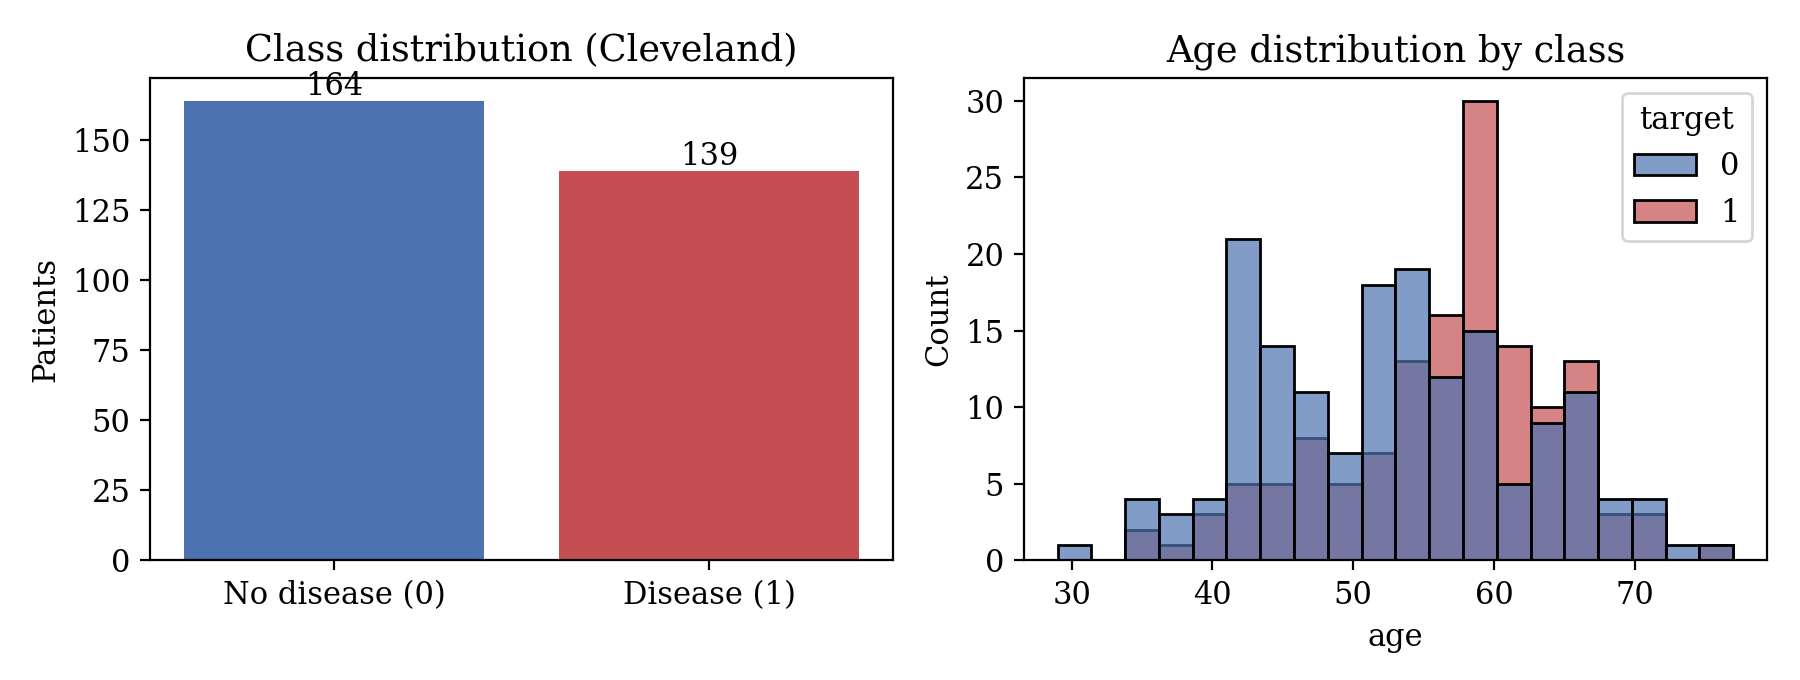
\includegraphics[width=0.85\textwidth]{figures/eda_cleveland.png}
\caption{Class balance and age distribution, Cleveland}
\end{figure}

\subsection{Pearson Correlation Feature Selection}
For each predictor x and the label y the Pearson coefficient is

\begin{equation}
r_{xy} = \frac{\operatorname{Cov}(x,y)}{\sigma_x\,\sigma_y}
\end{equation}
where Cov(x, y) measures how x and y vary together and the product of standard deviations normalises it to the range -1 to 1. Since \cite{r1} does not state a threshold, we make the rule explicit: a predictor is kept if \textbar{}r\_xy\textbar{} is at least 0.10, and if two kept predictors have \textbar{}r\textbar{} above 0.80 the one less correlated with the label is dropped. On Cleveland this removes chol, fbs; on the combined data chol, restecg. No pair of predictors exceeds 0.60, so the redundancy rule never fires (Fig. 2).

\begin{figure}[htbp]
\centering
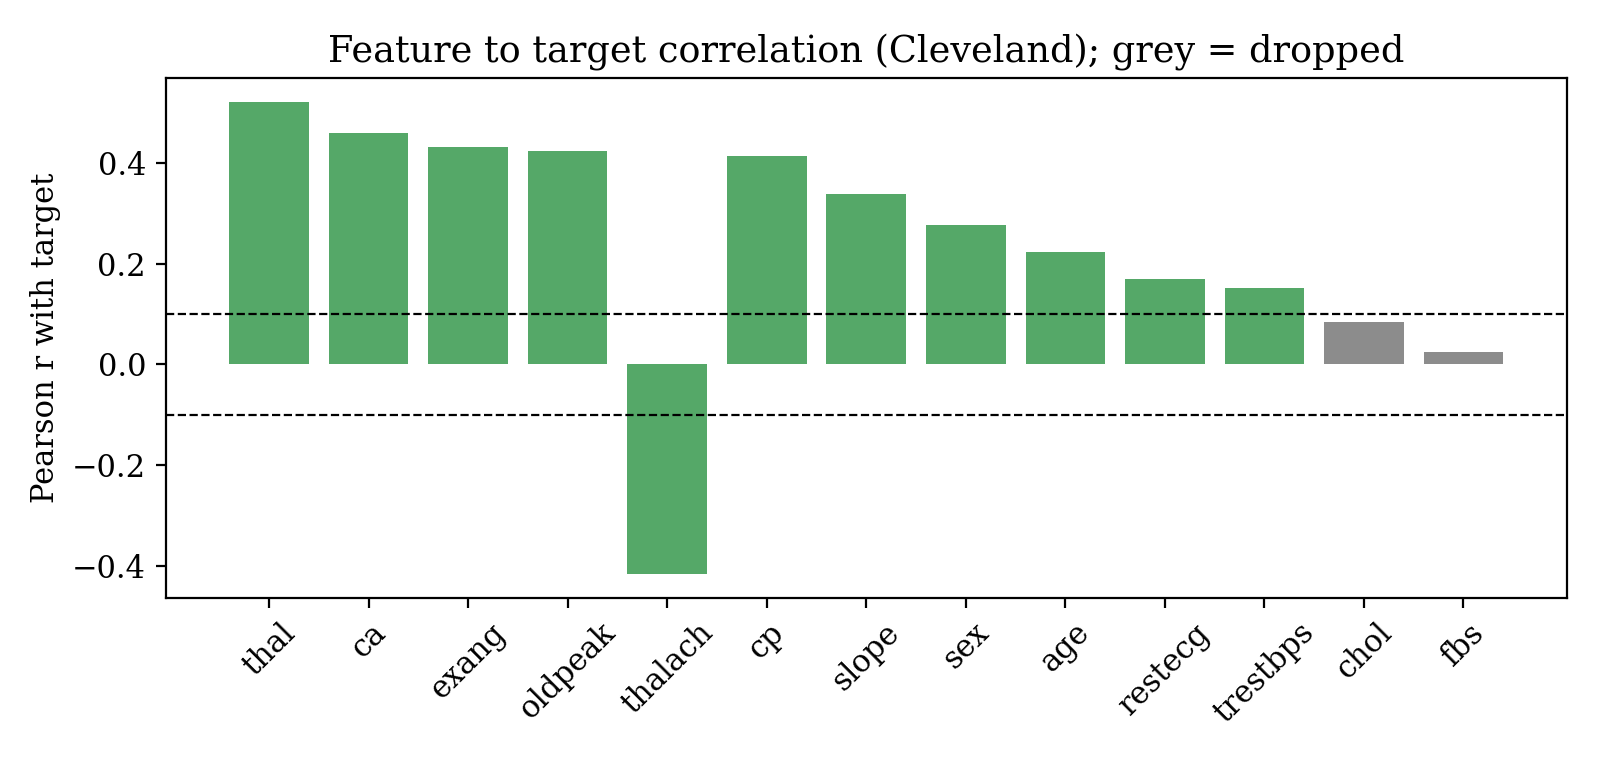
\includegraphics[width=0.85\textwidth]{figures/target_corr_cleveland.png}
\caption{Correlation of each attribute with the label on Cleveland; grey bars are dropped}
\end{figure}

\subsection{MinMax Normalisation}
Every kept attribute is mapped to 0 to 1 by x' = (x - x\_min)/(x\_max - x\_min), with x\_min and x\_max computed \textbf{on the training fold only} and applied to the test fold. This is implemented as a scikit-learn Pipeline so that no statistic of the test fold reaches the model; it is the one place where our protocol deliberately differs from the description in \cite{r1}.

\subsection{The MPBE Ensemble}
Four bagging ensembles are built, one per base learner: Decision Tree (CART, Gini), Random Forest (50 trees), Gaussian Naive Bayes and RBF SVM with Platt probabilities. Each ensemble holds 100 estimators trained on bootstrap resamples of the training fold. The prediction is the mean of the four bagged probabilities, thresholded at 0.5:

\begin{equation}
P_{\mathrm{MPBE}}(y=1\mid x)=\frac{1}{4}\sum_{k=1}^{4}\frac{1}{100}\sum_{b=1}^{100}P_{k,b}(y=1\mid x)
\end{equation}
The inner average over bootstrap models reduces the variance of each learner family; the outer average lets the families compensate for each other's errors. We read the 'mean score' aggregation of \cite{r1} as this soft average and include a hard voting ensemble for contrast.

\begin{figure}[htbp]
\centering
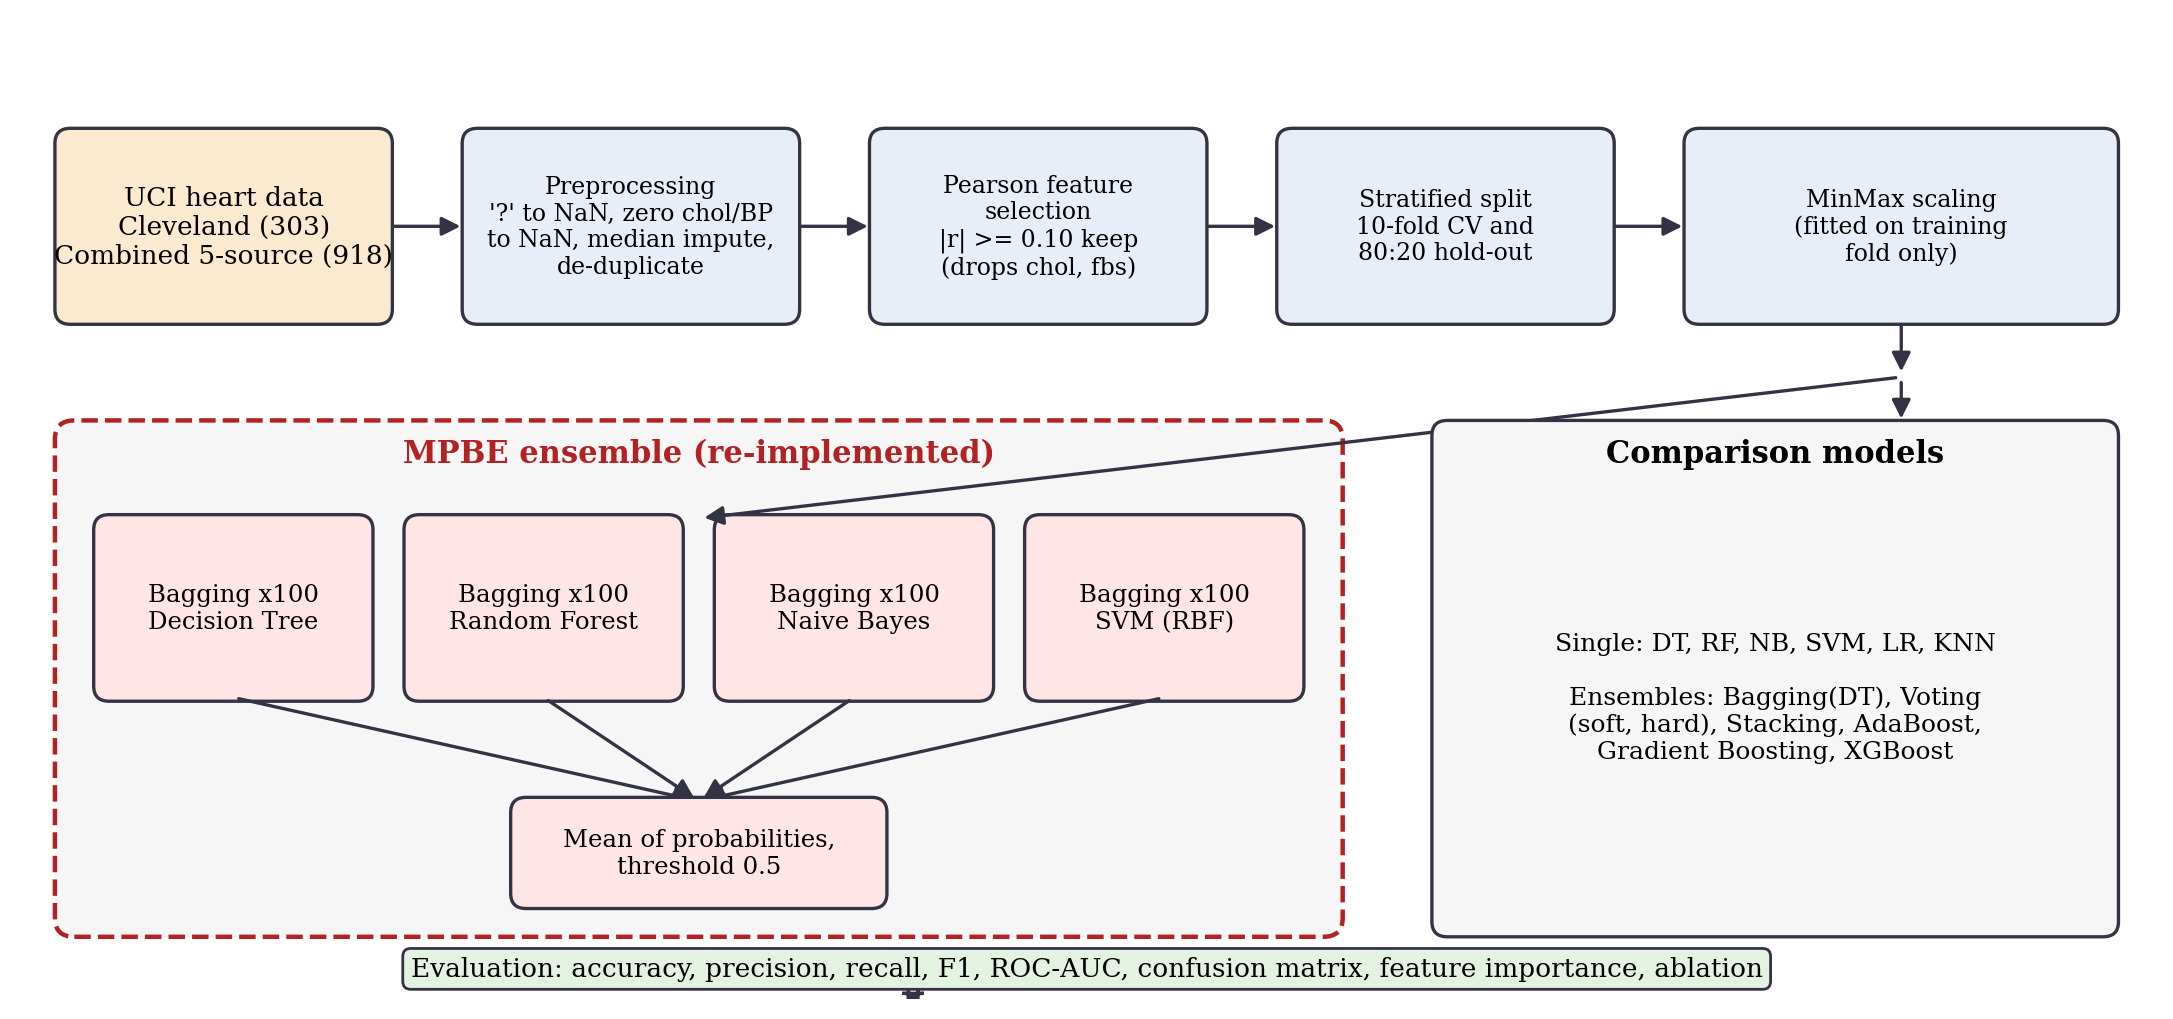
\includegraphics[width=1.00\textwidth]{figures/architecture.png}
\caption{Pipeline of the re-implemented MPBE model and the comparison branch}
\end{figure}

\subsection{Comparison Models and Protocol}
Six single models (DT, RF with 100 trees, NB, SVM, Logistic Regression, KNN with k = 7) and six ensembles are evaluated: homogeneous Bagging of 100 trees; soft and hard Voting over DT, RF, NB, SVM and LR; Stacking of DT, RF, NB and SVM with a logistic meta learner on 5 fold out-of-fold predictions; AdaBoost (100 stumps, learning rate 0.5); Gradient Boosting (100 trees, depth 3, rate 0.1); and XGBoost \cite{r25} (100 trees, depth 3, rate 0.1, subsample 0.9). Hyperparameters are default or lightly set and identical on both datasets so that the comparison isolates the ensemble design from tuning. All models use StratifiedKFold(10, shuffle, seed 42); a stratified 80:20 hold-out with the same seed provides confusion matrices and ROC curves. Metrics are accuracy, precision, recall, F1 and ROC-AUC.

\section{Results}
\subsection{Cleveland}
\begin{table}[htbp]
\centering
\caption{10-fold CV on Cleveland (11 selected attributes). Accuracy is mean and standard deviation over folds}
\scriptsize
\begin{tabular}{>{\raggedright\arraybackslash}p{0.353\textwidth}>{\raggedright\arraybackslash}p{0.200\textwidth}>{\raggedright\arraybackslash}p{0.141\textwidth}>{\raggedright\arraybackslash}p{0.129\textwidth}>{\raggedright\arraybackslash}p{0.106\textwidth}}
\hline
\textbf{Model} & \textbf{Accuracy (\%)} & \textbf{Recall (\%)} & \textbf{F1 (\%)} & \textbf{AUC} \\
\hline
Naive Bayes & 83.78 $\pm$ 6.10 & 79.07 & 81.66 & 0.902 \\
Stacking (LR meta) & 83.78 $\pm$ 6.79 & 79.07 & 81.55 & 0.915 \\
AdaBoost & 83.45 $\pm$ 5.44 & 79.84 & 81.65 & 0.910 \\
Voting (soft) & 82.84 $\pm$ 5.09 & 79.12 & 80.97 & 0.910 \\
Logistic Regression & 82.80 $\pm$ 7.01 & 78.35 & 80.69 & 0.908 \\
Voting (hard) & 82.48 $\pm$ 6.00 & 77.64 & 80.31 & n/a \\
MPBE (proposed, replicated) & 82.46 $\pm$ 6.41 & 76.92 & 80.03 & 0.912 \\
Random Forest & 82.17 $\pm$ 4.26 & 77.69 & 80.03 & 0.897 \\
SVM (RBF) & 82.15 $\pm$ 6.24 & 77.58 & 79.92 & 0.903 \\
XGBoost & 81.85 $\pm$ 4.72 & 76.98 & 79.69 & 0.899 \\
Gradient Boosting & 80.49 $\pm$ 5.67 & 76.87 & 78.30 & 0.874 \\
KNN (k=7) & 79.87 $\pm$ 5.02 & 79.07 & 78.17 & 0.877 \\
Bagging (DT, 100) & 79.83 $\pm$ 4.93 & 74.07 & 76.92 & 0.894 \\
Decision Tree & 77.17 $\pm$ 7.19 & 72.58 & 74.29 & 0.768 \\
\hline
\end{tabular}
\end{table}

\begin{figure}[htbp]
\centering
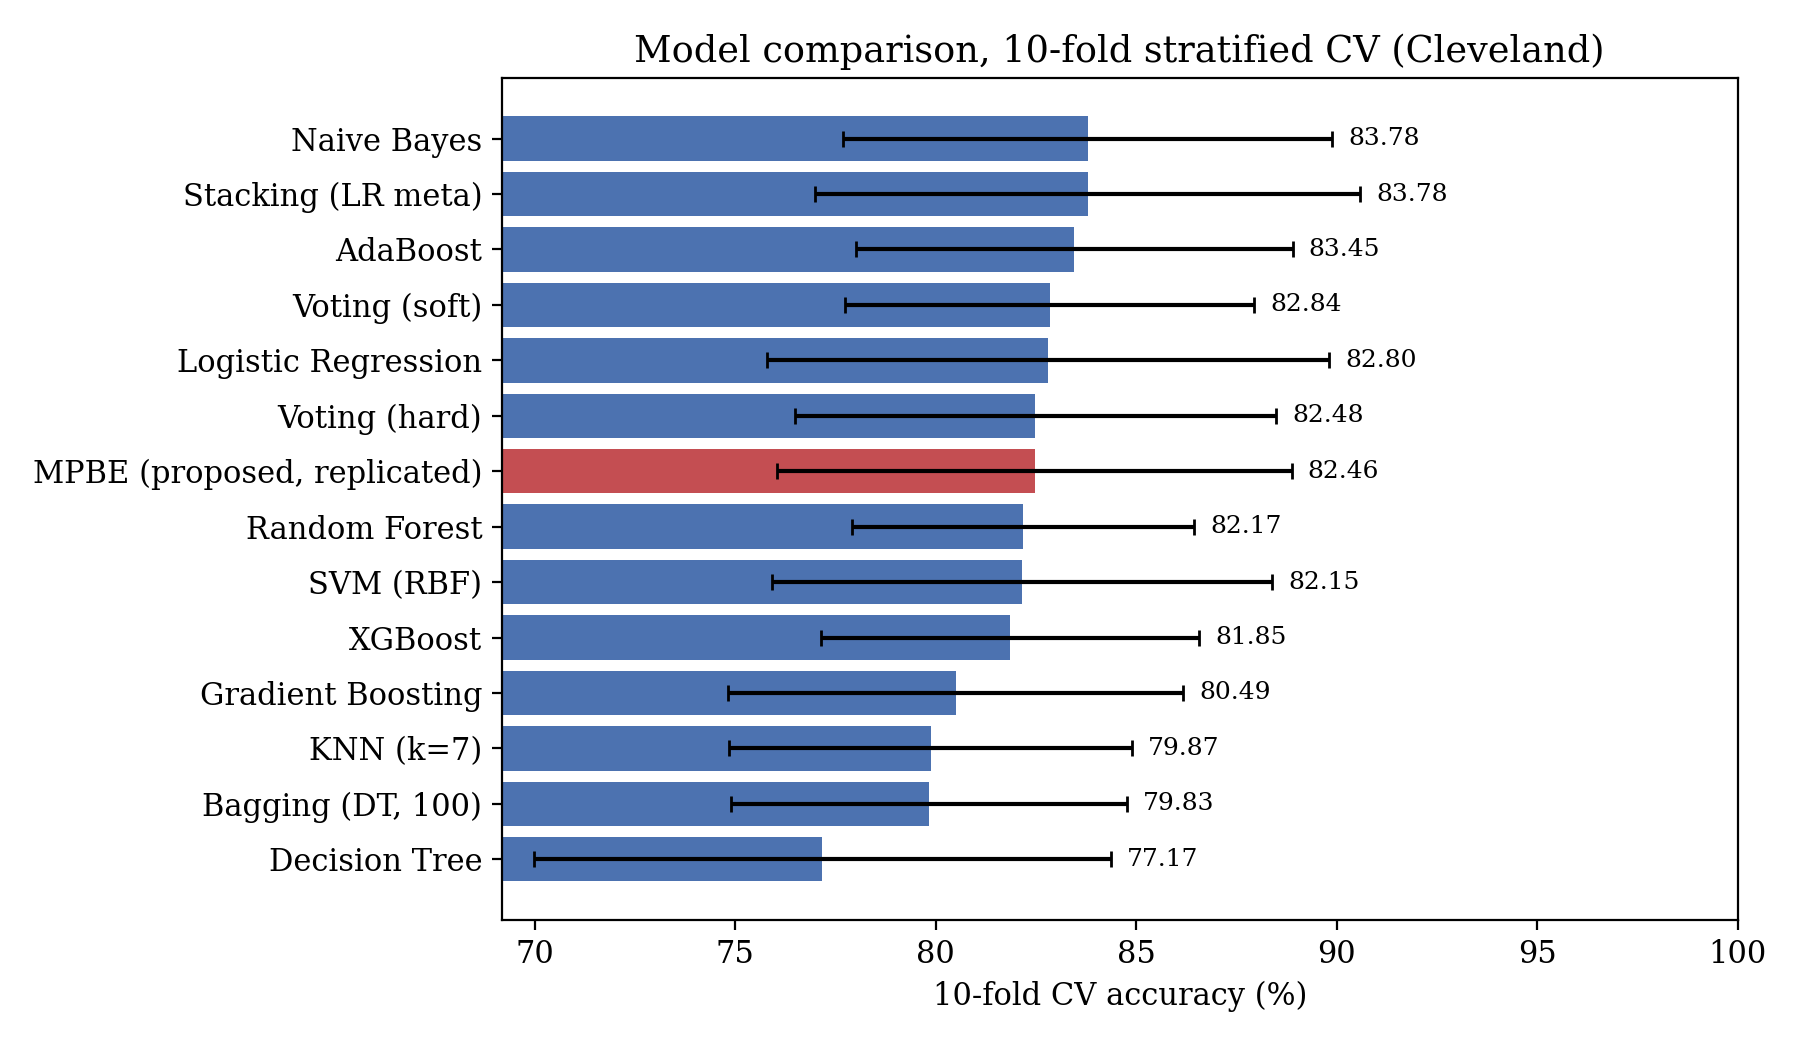
\includegraphics[width=0.85\textwidth]{figures/cv_accuracy_cleveland.png}
\caption{10-fold CV accuracy with standard deviation on Cleveland (MPBE in red)}
\end{figure}

MPBE obtains 82.46 $\pm$ 6.41\% accuracy and AUC 0.912, the second highest AUC of the fourteen models, and ranks 7th by accuracy behind Naive Bayes and Stacking (83.78\%), AdaBoost, soft Voting and Logistic Regression. All of these lie within one fold standard deviation (5 to 7 points on folds of 30 patients) of each other. The informative gaps are below: the single Decision Tree (77.2\%) and homogeneous tree Bagging (79.8\%) trail MPBE by 5.3 and 2.6 points, so mixing four learner families is worth about 2.6 points over bagging one family, which is the central claim of \cite{r1}. On the hold-out split MPBE scores 86.89\% with recall 92.86\% and AUC 0.958 (Fig. 5); Random Forest is best there at 90.2\%, illustrating how a 61 patient test set reorders models by one or two patients.

\begin{figure}[htbp]
\centering
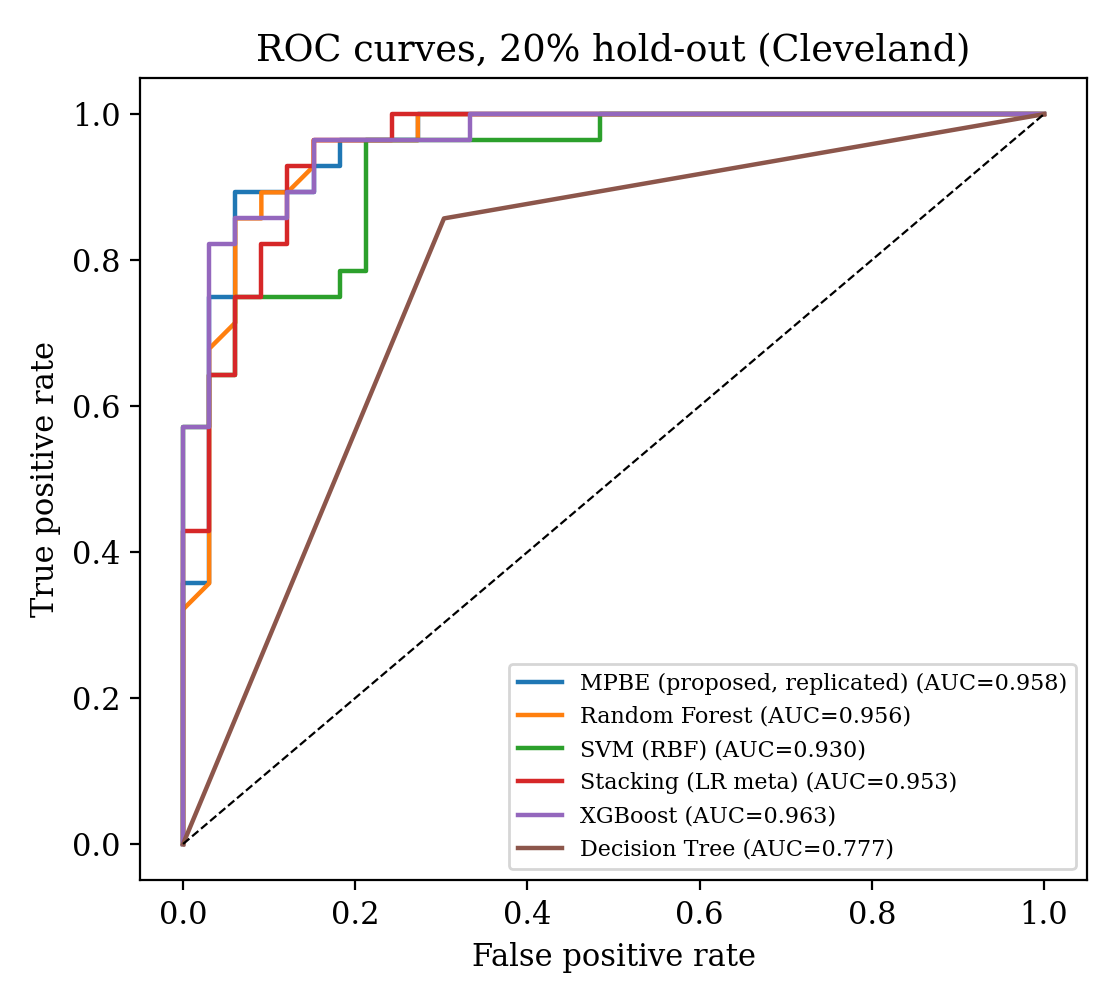
\includegraphics[width=0.55\textwidth]{figures/roc_cleveland.png}
\caption{ROC curves on the Cleveland hold-out split}
\end{figure}

\subsection{Combined Dataset}
\begin{table}[htbp]
\centering
\caption{10-fold CV on the combined 5 source dataset (918 records)}
\scriptsize
\begin{tabular}{>{\raggedright\arraybackslash}p{0.353\textwidth}>{\raggedright\arraybackslash}p{0.200\textwidth}>{\raggedright\arraybackslash}p{0.141\textwidth}>{\raggedright\arraybackslash}p{0.129\textwidth}>{\raggedright\arraybackslash}p{0.106\textwidth}}
\hline
\textbf{Model} & \textbf{Accuracy (\%)} & \textbf{Recall (\%)} & \textbf{F1 (\%)} & \textbf{AUC} \\
\hline
MPBE (proposed, replicated) & 80.84 $\pm$ 3.53 & 83.29 & 82.81 & 0.884 \\
Random Forest & 80.73 $\pm$ 2.93 & 84.47 & 82.90 & 0.870 \\
Gradient Boosting & 80.72 $\pm$ 2.90 & 84.65 & 82.89 & 0.878 \\
Voting (hard) & 80.51 $\pm$ 3.23 & 82.10 & 82.38 & n/a \\
Stacking (LR meta) & 80.40 $\pm$ 3.49 & 83.69 & 82.56 & 0.883 \\
Logistic Regression & 80.19 $\pm$ 3.35 & 82.70 & 82.24 & 0.876 \\
Voting (soft) & 80.19 $\pm$ 3.65 & 82.30 & 82.18 & 0.877 \\
Naive Bayes & 80.18 $\pm$ 2.90 & 79.15 & 81.52 & 0.874 \\
AdaBoost & 80.18 $\pm$ 3.67 & 82.89 & 82.23 & 0.878 \\
SVM (RBF) & 79.75 $\pm$ 3.37 & 84.86 & 82.31 & 0.879 \\
XGBoost & 79.52 $\pm$ 2.54 & 83.08 & 81.75 & 0.878 \\
Bagging (DT, 100) & 79.52 $\pm$ 3.25 & 82.09 & 81.62 & 0.851 \\
KNN (k=7) & 78.22 $\pm$ 3.25 & 81.30 & 80.57 & 0.852 \\
Decision Tree & 70.81 $\pm$ 4.16 & 71.24 & 72.86 & 0.712 \\
\hline
\end{tabular}
\end{table}

\begin{figure}[htbp]
\centering
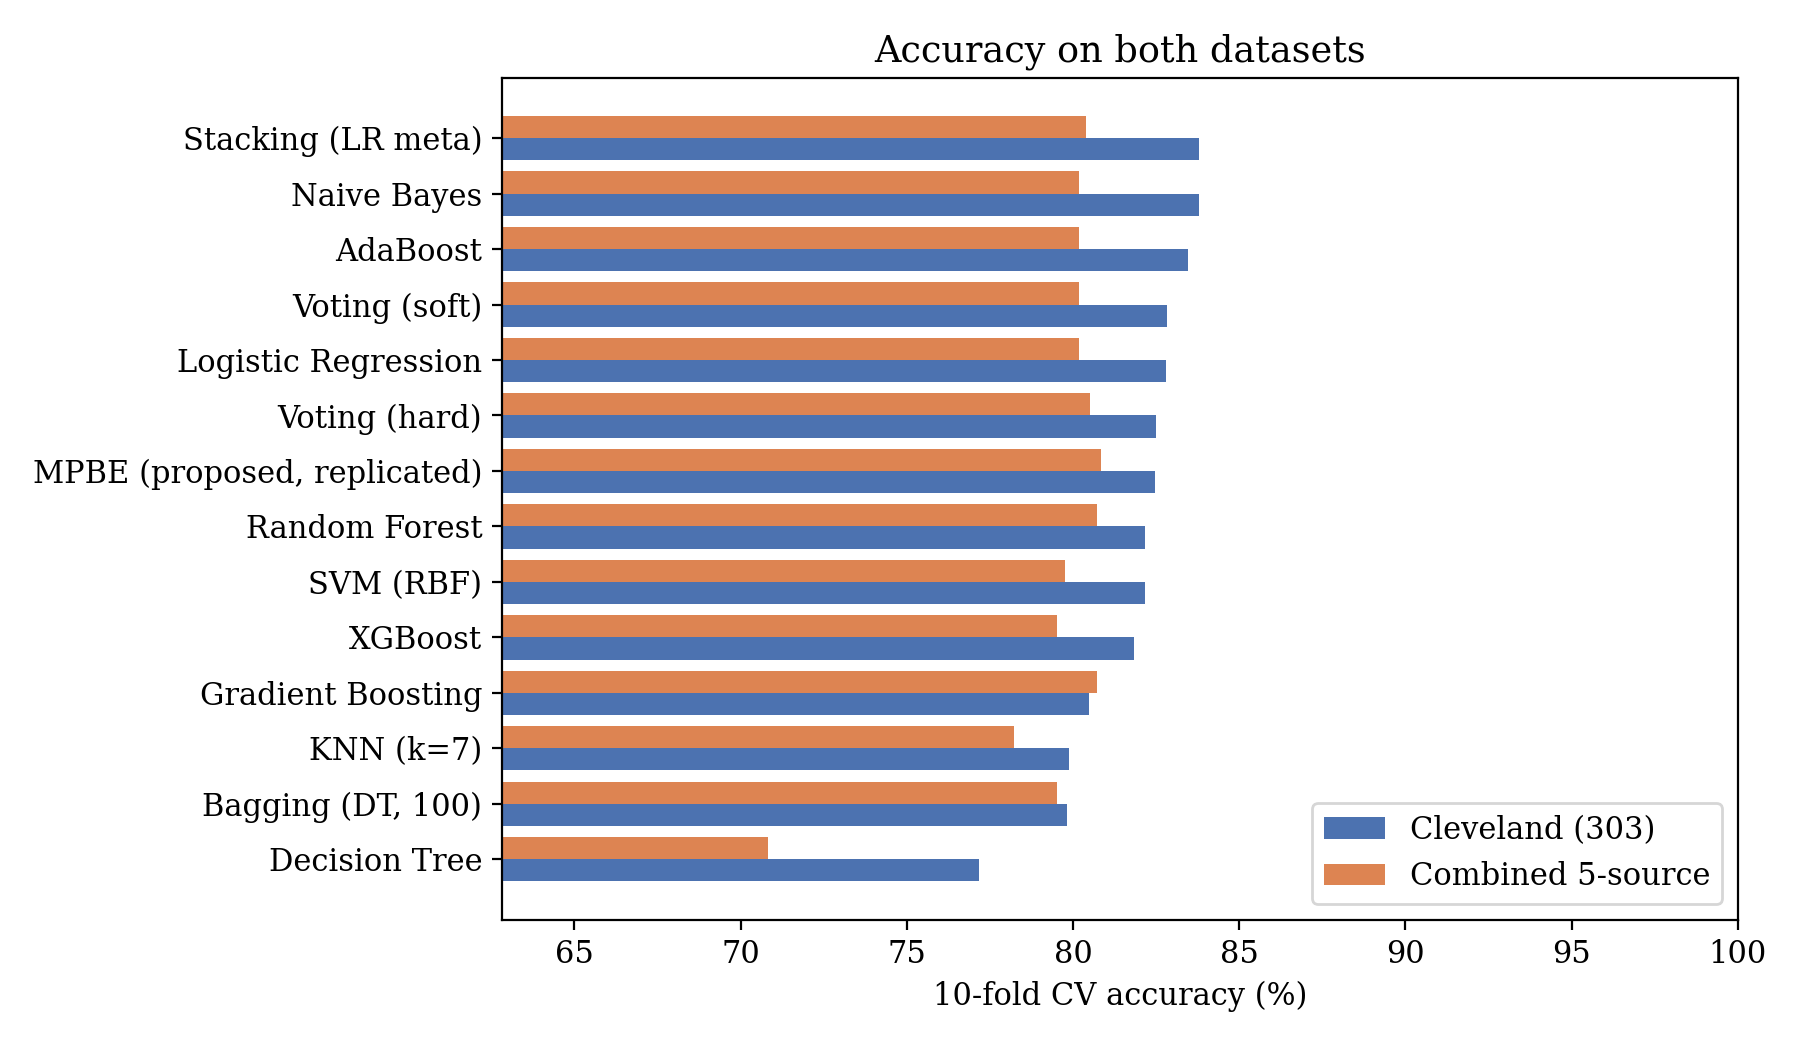
\includegraphics[width=0.85\textwidth]{figures/cross_dataset.png}
\caption{10-fold CV accuracy of every model on both datasets}
\end{figure}

On the combined population MPBE is \textbf{first} by accuracy (80.84 $\pm$ 3.53\%) and ties Stacking for the best AUC (0.884); it is also first on the hold-out split (82.07\%, recall 85.29\%). Fold standard deviations fall to about 3 points, so this ranking is more reliable than the Cleveland one. Every model loses accuracy on the harder data (Fig. 6), the Decision Tree most (to 70.8\%) and MPBE least (about 1.6 points), which is the property one wants from a model meant to run across hospitals.

\begin{figure}[htbp]
\centering
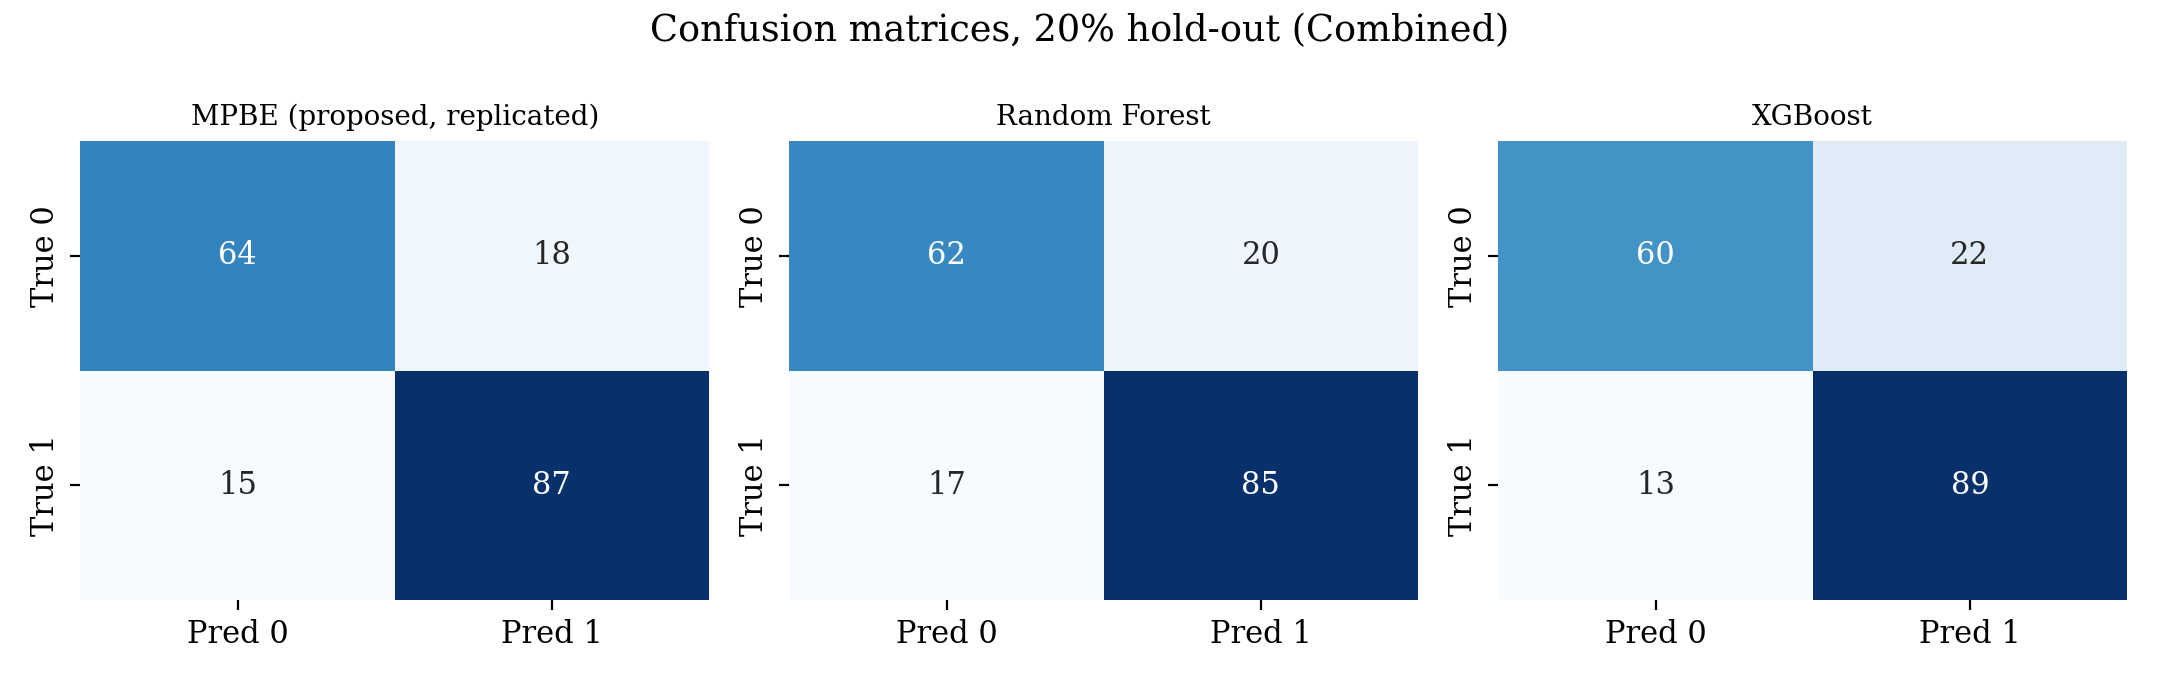
\includegraphics[width=0.95\textwidth]{figures/cm_combined.png}
\caption{Confusion matrices on the combined hold-out split}
\end{figure}

\subsection{Ablation of Feature Selection}
\begin{table}[htbp]
\centering
\caption{MPBE with and without Pearson selection (10-fold CV)}
\scriptsize
\begin{tabular}{>{\raggedright\arraybackslash}p{0.186\textwidth}>{\raggedright\arraybackslash}p{0.186\textwidth}>{\raggedright\arraybackslash}p{0.186\textwidth}>{\raggedright\arraybackslash}p{0.186\textwidth}>{\raggedright\arraybackslash}p{0.186\textwidth}}
\hline
\textbf{Dataset} & \textbf{Attributes} & \textbf{Accuracy (\%)} & \textbf{F1 (\%)} & \textbf{AUC} \\
\hline
Cleveland & 11 selected & 82.46 & 80.03 & 0.912 \\
Cleveland & all 13 & 82.46 & 80.14 & 0.909 \\
Combined & 11 selected & 80.84 & 82.81 & 0.884 \\
Combined & all 13 & 81.05 & 82.89 & 0.888 \\
\hline
\end{tabular}
\end{table}

Dropping the two weakest attributes moves accuracy by less than half a point and AUC by at most 0.003. The selection step is harmless and yields a marginally cheaper screening model, but it is not the source of any accuracy gain, in agreement with \cite{r7,r9}.

\subsection{Feature Importance}
\begin{figure}[htbp]
\centering
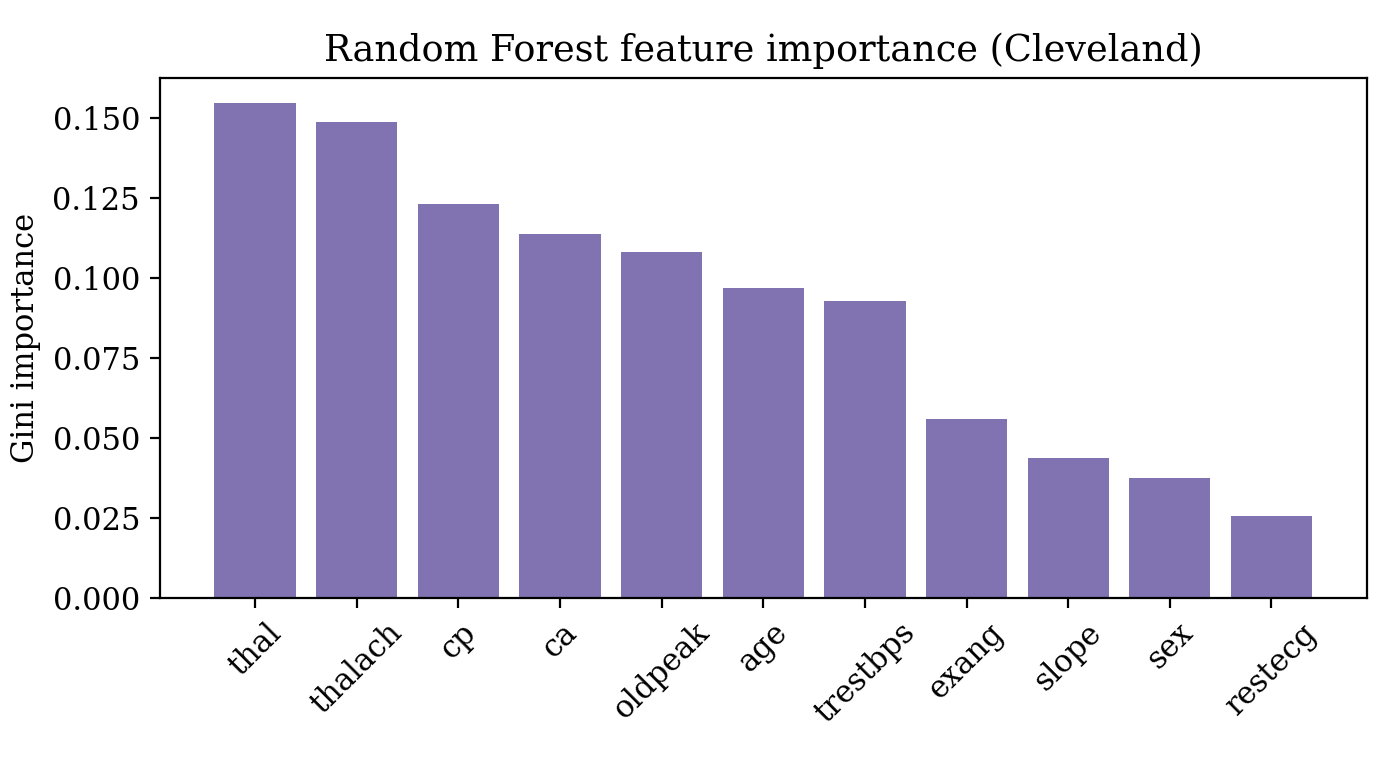
\includegraphics[width=0.75\textwidth]{figures/importance_cleveland.png}
\caption{Random Forest Gini importance on Cleveland}
\end{figure}

Random Forest importances rank thal, thalach, cp, ca and oldpeak highest on Cleveland; on the combined data cp, age, thalach and oldpeak dominate because thal and ca are mostly imputed outside Cleveland. Chest pain type, maximum heart rate and exercise ST depression are therefore the attributes a screening protocol should record first, consistent with \cite{r15,r16}.

\section{Discussion}
Three conclusions follow. \textbf{(1) The 95.33\% of \cite{r1} does not survive a leakage free protocol.} Under stratified 10-fold cross validation no model in this study exceeds 84\% mean accuracy on Cleveland, in line with \cite{r8,r9,r10,r21}. The original figure is most plausibly a single favourable split with scaling and selection applied to the whole dataset. \textbf{(2) The design of MPBE is nevertheless sound.} Heterogeneous bagging beats bagging a single learner family by 2.6 points on Cleveland and 1.3 on the combined data, and it is the most stable model across the two populations. \textbf{(3) Ensemble gains over strong single learners are small on this data.} Logistic Regression and Naive Bayes are within a point of every ensemble on Cleveland; the practical value of MPBE appears when the data become heterogeneous and noisy, where variance reduction matters. Limitations are the modest dataset sizes, median imputation of attributes missing by design in three sources, and the absence of hyperparameter tuning, which was deliberate. Future work should tune the decision threshold for recall, add SHAP based explanations, and validate on a local Indian cohort.

\section{Conclusion}
We re-implemented the MPBE heterogeneous bagging ensemble and evaluated it against thirteen alternatives on two datasets under a strict protocol. MPBE reaches 82.46\% accuracy (AUC 0.912) on Cleveland and is the best model on a combined 918 patient dataset (80.84\%, AUC 0.884). The reported 95.33\% could not be reproduced, the Pearson selection step contributes under half a point, and heterogeneous bagging is a robust default for tabular clinical screening. All code and figures are provided for verification.

\begin{thebibliography}{99}
\bibitem{r1} P. Muthulakshmi, M. Parveen and P. Rajeswari, "Prediction of Heart Disease using Ensemble Learning," Indian Journal of Science and Technology, vol. 16, no. 20, pp. 1469-1476, 2023. doi: 10.17485/IJST/v16i20.2279
\bibitem{r2} M. Pal, S. Parija, G. Panda, K. Dhama and R. K. Mohapatra, "Risk prediction of cardiovascular disease using machine learning classifiers," Open Medicine, vol. 17, no. 1, pp. 1100-1113, 2022. doi: 10.1515/med-2022-0508
\bibitem{r3} A. Alqahtani, S. Alsubai, M. Sha, L. Vilcekova and T. Javed, "Cardiovascular Disease Detection using Ensemble Learning," Computational Intelligence and Neuroscience, vol. 2022, art. 5267498, pp. 1-9, 2022. doi: 10.1155/2022/5267498
\bibitem{r4} I. D. Mienye, Y. Sun and Z. Wang, "An improved ensemble learning approach for the prediction of heart disease risk," Informatics in Medicine Unlocked, vol. 20, art. 100402, 2020. doi: 10.1016/j.imu.2020.100402
\bibitem{r5} A. U. Haq, J. P. Li, M. H. Memon, S. Nazir and R. Sun, "A Hybrid Intelligent System Framework for the Prediction of Heart Disease Using Machine Learning Algorithms," Mobile Information Systems, vol. 2018, art. 3860146, pp. 1-21, 2018. doi: 10.1155/2018/3860146
\bibitem{r6} B. P. Doppala, D. Bhattacharyya, M. Janarthanan and N. Baik, "A Reliable Machine Intelligence Model for Accurate Identification of Cardiovascular Diseases Using Ensemble Techniques," Journal of Healthcare Engineering, vol. 2022, art. 2585235, 2022. doi: 10.1155/2022/2585235
\bibitem{r7} M. A. Alim, S. Habib, Y. Farooq and A. Rafay, "Robust Heart Disease Prediction: A Novel Approach based on Significant Feature and Ensemble learning Model," in Proc. 3rd Int. Conf. on Computing, Mathematics and Engineering Technologies (iCoMET), 2020, pp. 1-5. doi: 10.1109/iCoMET48670.2020.9074135
\bibitem{r8} S. Mohan, C. Thirumalai and G. Srivastava, "Effective Heart Disease Prediction Using Hybrid Machine Learning Techniques," IEEE Access, vol. 7, pp. 81542-81554, 2019. doi: 10.1109/ACCESS.2019.2923707
\bibitem{r9} C. B. C. Latha and S. C. Jeeva, "Improving the accuracy of prediction of heart disease risk based on ensemble classification techniques," Informatics in Medicine Unlocked, vol. 16, art. 100203, 2019. doi: 10.1016/j.imu.2019.100203
\bibitem{r10} V. Shorewala, "Early detection of coronary heart disease using ensemble techniques," Informatics in Medicine Unlocked, vol. 26, art. 100655, 2021. doi: 10.1016/j.imu.2021.100655
\bibitem{r11} M. M. Ali, B. K. Paul, K. Ahmed, F. M. Bui, J. M. W. Quinn and M. A. Moni, "Heart disease prediction using supervised machine learning algorithms: Performance analysis and comparison," Computers in Biology and Medicine, vol. 136, art. 104672, 2021. doi: 10.1016/j.compbiomed.2021.104672
\bibitem{r12} D. Shah, S. Patel and S. K. Bharti, "Heart Disease Prediction using Machine Learning Techniques," SN Computer Science, vol. 1, no. 6, art. 345, 2020. doi: 10.1007/s42979-020-00365-y
\bibitem{r13} R. Bharti, A. Khamparia, M. Shabaz, G. Dhiman, S. Pande and P. Singh, "Prediction of Heart Disease Using a Combination of Machine Learning and Deep Learning," Computational Intelligence and Neuroscience, vol. 2021, art. 8387680, pp. 1-11, 2021. doi: 10.1155/2021/8387680
\bibitem{r14} T. Karadeniz, G. Tokdemir and H. H. Maras, "Ensemble Methods for Heart Disease Prediction," New Generation Computing, vol. 39, no. 3, pp. 569-581, 2021.
\bibitem{r15} J. P. Li, A. U. Haq, S. U. Din, J. Khan, A. Khan and A. Saboor, "Heart Disease Identification Method Using Machine Learning Classification in E-Healthcare," IEEE Access, vol. 8, pp. 107562-107582, 2020.
\bibitem{r16} I. D. Mienye and N. Jere, "Optimized Ensemble Learning Approach with Explainable AI for Improved Heart Disease Prediction," Information, vol. 15, no. 7, art. 394, 2024. doi: 10.3390/info15070394
\bibitem{r17} D. Asif, M. Bibi, M. S. Arif and A. Mukheimer, "Enhancing Heart Disease Prediction through Ensemble Learning Techniques with Hyperparameter Optimization," Algorithms, vol. 16, no. 6, art. 308, 2023. doi: 10.3390/a16060308
\bibitem{r18} N. Chandrasekhar and S. Peddakrishna, "Enhancing Heart Disease Prediction Accuracy through Machine Learning Techniques and Optimization," Processes, vol. 11, no. 4, art. 1210, 2023. doi: 10.3390/pr11041210
\bibitem{r19} G. N. Ahmad, H. Fatima, S. Ullah, A. S. Saidi and Imdadullah, "Efficient Medical Diagnosis of Human Heart Diseases Using Machine Learning Techniques With and Without GridSearchCV," IEEE Access, vol. 10, pp. 80151-80173, 2022. doi: 10.1109/ACCESS.2022.3165792
\bibitem{r20} G. Narasimhan and A. Victor, "Grey wolf optimized stacked ensemble machine learning based model for enhanced efficiency and reliability of predicting early heart disease," Automatika, vol. 65, no. 3, pp. 749-762, 2024. doi: 10.1080/00051144.2024.2317098
\bibitem{r21} A. Adekoya, F. Saeed, W. Ghaban and S. N. Qasem, "Ensemble learning approach with explainable AI for improved heart disease prediction," Frontiers in Pharmacology, vol. 16, art. 1654681, 2025. doi: 10.3389/fphar.2025.1654681
\bibitem{r22} A. Janosi, W. Steinbrunn, M. Pfisterer and R. Detrano, "Heart Disease," UCI Machine Learning Repository, 1988. doi: 10.24432/C52P4X
\bibitem{r23} "Statlog (Heart)," UCI Machine Learning Repository. doi: 10.24432/C57303
\bibitem{r24} F. Pedregosa et al., "Scikit-learn: Machine Learning in Python," Journal of Machine Learning Research, vol. 12, pp. 2825-2830, 2011.
\bibitem{r25} T. Chen and C. Guestrin, "XGBoost: A Scalable Tree Boosting System," in Proc. 22nd ACM SIGKDD Int. Conf. on Knowledge Discovery and Data Mining, 2016, pp. 785-794. doi: 10.1145/2939672.2939785
\end{thebibliography}

\end{document}
